
\chapter{Organizing Committee}

\begin{description}

\item[AB3C President:] Glória R Franco (UFMG)

\item[AB3C Vice President:] Alan M Durham (USP)


\item[AB3C Secretaries]:

\begin{itemize}
 \item Marcelo Brandão (Unicamp) 
\item  Ney Lemke (Unesp)
\end{itemize}

\item[AB3C Financial Department]:

\begin{itemize}
\item Priscila Grynberg (Embrapa)
\item Fábio Passetti (Fiocruz)
\end{itemize}

\item[Poster Session Organizers]:

\begin{itemize}
\item Mainá Bitar (UFMG)
\item Nicole Scherer (INCA)
\end{itemize}

\item[Local Committee]:

\begin{itemize}
\item Vasco Azevedo (UFMG)
\item Liza Felicori (UFMG)
\item Rafaela Ferreira (UFMG)
\item Lucas Bleicher (UFMG)
\item Mainá Bitar (UFMG/QIMR)
\end{itemize}
\end{description}
\newpage
\chapter{Introduction}
The Brazilian Association of Bioinformatics and Computational Biology (AB3C) is
a scientific society funded in July 12th 2004.
Since its creation, AB3C has been responsible for the annual conference entitled
“X-Meeting” which is the main Bioinformatics and Computation Biology event in
Brazil.This year its 12th edition occurred in Belo Horizonte MG.

	
Bioinformatics is now a strategic area for Brazil and all Latin America and,
therefore, it is also strategic to the development of Science, Technology and
Economy. The X-Meeting is a Brazilian event with international reach which has
an average of 400 participants. The Conference is an opportunity for students,
researchers and companies to interact and difuse knowledge. The AB3C has been a
pioneer society in the field of Bioinformatics in Brazil and we have a history
of ten past very productive meetings.

\begin{figure}[h]
    \begin{center}
  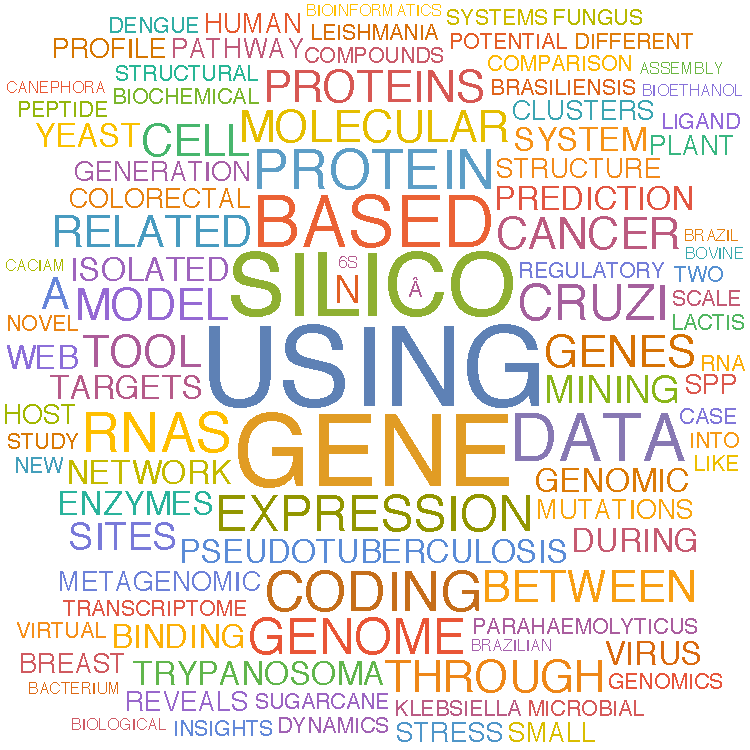
\includegraphics[scale=0.7]{wordcloud}
\end{center}
\caption{Word Cloud for the words used on the Conference Papers Titles}
\end{figure}